% Chapter X

\chapter{Funzioni trigonometriche} % Chapter title

\label{ch:trigonometria} % For referencing the chapter elsewhere, use \autoref{ch:name}

\section{Radianti}

Sia $\gamma$ una circonferenza di raggio $1$ (detta circonferenza goniometrica) il cui centro $O$ è anche l'origine di un sistema di assi cartesiani e sia $A$ il punto $(1,0)$.
Partendo da $A$ percorriamo la circonferenza in senso antiorario oppure in senso orario.
Sia $x$ un numero reale, denotiamo con $P_x$ il punto su $\gamma$ che si ottiene percorrendo la circonferenza a partire dal punto $A$ per un arco di lunghezza $|x|$, in senso antorario se $x \geq 0$, oppure in senso orario se $x<0$.
Il punto $P_x$ individua un angolo nel piano avente vertice $O$ e delimitatio dalle semirette nel piano uscenti da $O$ e passanti per $A$ e per $P_x$.
Il numero reale $x$ rappresenta la misura dell'angolo in radianti.

\begin{wrapfigure}{r}{0.45\textwidth}
  \begin{center}
    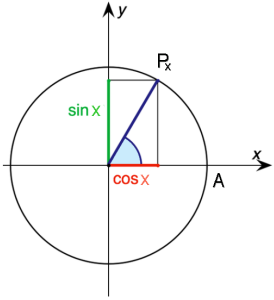
\includegraphics[width=0.42\textwidth]{gfx/4/circonferenza.png}
  \end{center}
  \caption{Circonferenza goniometrica}\label{fig:goniometrica}
\end{wrapfigure}

La relazione tra radianti e gradi è data da:
\[\frac{\gamma_{\text{radianti}}}{2\pi}=\frac{\gamma_{\text{gradi}}}{360}\]

Osserviamo che l'incremento della lunghezza $x$ di $2\pi$ corrisponde a compiere un intero giro sulla circonferenza in senso antiorario ritornando al punto $P_x$ (così come decrementare di $2\pi$ la lunghezza $x$). Quindi si ha:
\[P_{x\pm k2\pi}=P_x \qquad \forall x \in \R, k \in \N\]

\section{Le funzioni seno e coseno}
Una funzione $f:\R \in \R$ è detta periodica di periodo $T$, $T>0$ se:
\[f(x+T)=f(x) \forall x \in \R\]
La caratteristica fondamentale delle funzioni periodiche è che i suoi valori si ripetono dopo intervalli di ampiezza $T$.

\subsection{Simmetria}
Indichiamo con $\cos x$ e con $\sin x$ rispettivamente l'ascissa e l'ordinata del punto $P_x$. Le funzioni $y=\cos x$ e $y=\sin x$ sono definite su $\R$ a valori nell'intervallo $[-1,1]$, sono periodiche di minimo periodo $2\pi$ e soddisfano la relazione:
\[\sin^2 x + \cos^2 x = 1\]

\subsection{Monotonia} Per la periodicità di seno e coseno ci basta studiarne le proprietà nell'intervallo $[0,2\pi]$. Dalle definizioni segue subito che la funzione seno è dispari e la funzione coseno è pari; inoltre la funzione coseno è strettamente decrescente in $[0,\pi]$ e strettamente crescente in $[\pi,2\pi]$. La funzione seno è strettamente crescente in $[0,\frac{\pi}{2}] \cup [\frac{3}{2}\pi,2\pi)$ e strettamente decrescente in $[\frac{\pi}{2},\frac{3}{2}\pi]$.

\begin{figure}[H]
{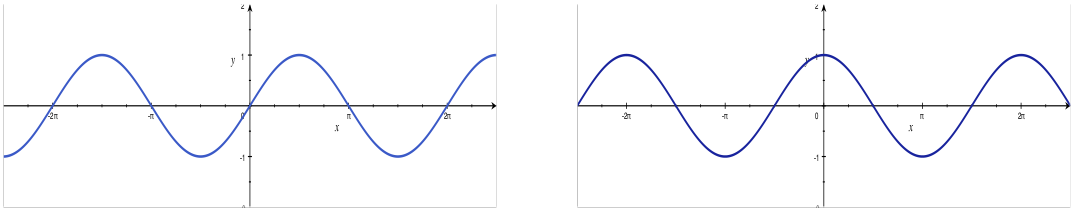
\includegraphics[width=1\linewidth]{gfx/4/senocoseno.png}}
\caption{Grafico delle funzioni: seno e coseno}\label{fig:seno-coseno}
\end{figure}

\subsection{Formule trigonometriche}
\subsubsection{Formule di addizione e sottrazione}
\[\sin(\alpha\pm\beta)=\sin(\alpha)\cos(\beta)\pm\cos(\alpha)\sin(\beta)\]
\[\cos(\alpha\pm\beta)=\cos(\alpha)\cos(\beta)\mp\sin(\alpha)\sin(\beta)\]
\subsubsection{Formule di duplicazione}
\[\sin(2x)=2\sin x\cos x\]
\[\cos(2x)=2\cos^2 x - 1\]
\subsubsection{Formule di potenza}
\[(\sin x)^2 = \sin^2 x= \frac{1-\cos(2x)}{2}\]
\[(\cos x)^2 = \cos^2 x= \frac{1+\cos(2x)}{2}\]
\subsubsection{Formule di bisezione}
\[\sin(\frac{x}{2})=\sqrt{\frac{1-\cos x}{2}} \qquad 0<x\leq 2\pi\]
\[\cos(\frac{x}{2})=\sqrt{\frac{1+\cos x}{2}} \qquad -\pi<x\leq \pi\]
\subsubsection{Formule di prostaferesi}
\[\sin x -\sin y=2\sin(\frac{x-y}{2})\cos(\frac{x+y}{2})\]
\[\cos x -\cos y=-2\cos(\frac{x-y}{2})\sin(\frac{x+y}{2})\]


\[\cos(x+\pi)=-\cos x \qquad \sin(x+\pi)=-\sin x\]
\[\cos(x+\frac{\pi}{2})=-\sin x \qquad \sin(x+\frac{\pi}{2})=\cos x \]

\section{La funzione tangente}
\begin{wrapfigure}{r}{0.45\textwidth}
  \begin{center}
    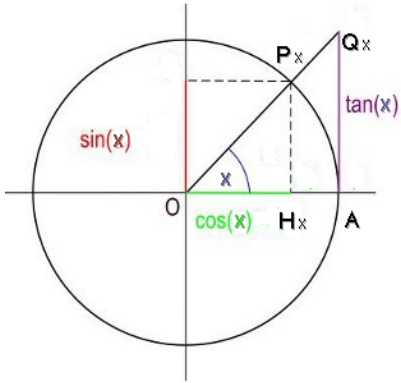
\includegraphics[width=0.42\textwidth]{gfx/4/tangente.png}
  \end{center}
  \caption{Tangente.}\label{fig:circo-tangente}
\end{wrapfigure}

La funzione tangente è:
\[\tan x = \frac{\sin x}{\cos x}\]
Definita nei punti di $\R$ diversi da $\frac{\pi}{2} +k\pi,k\in\Z$ e, come vedremo in seguito, ha immagine $\R$.
La funzione tangente è periodica per: $(x)=\tan(x+k\pi)$ per $k\in \Z$ cioè $\tan(x)$ è periodica di minimo periodo $T=\pi$.

Nella \autoref{fig:circo-tangente} è evidenziata la tangente nel punto $(A,Q_x=\tan(x))$.

\subsection{Simmetria}
Dalle proprietà di simmetria delle funzioni seno e coseno, si deduce che la funzione tangente è dispari: il rapporto di una funzione pari e di una funzione dispari è dispari.

\subsection{Monotonia}
La funzione tangente è strettamente crescente in ogni intervallo $(\frac{-\pi}{2}+k\pi,\frac{\pi}{2}+k\pi), k\in \Z$

\begin{figure}[H]
{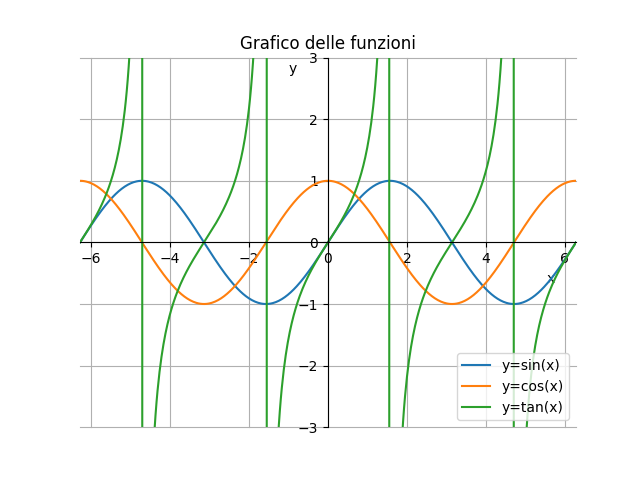
\includegraphics[width=.9\linewidth]{gfx/4/trigonometriche.png}}
\caption{Funzioni trigonometriche}\label{fig:trigonometriche}
\end{figure}

\section{Funzioni trigonometriche inverse}
Le funzioni trigonometriche inverse sono definite come, il dominio della funzione di partenza è stato ristretto per permettere l'inversione della funzione.

\[\arcsin x = f^{-1}(x) \qquad f(x)=\sin(x) \qquad x\in [\frac{-\pi}{2}, \frac{\pi}{2}]\]
\[\arccos x = f^{-1}(x) \qquad f(x)=\cos(x) \qquad x\in [0, \pi]\]
\[\arctan x = f^{-1}(x) \qquad f(x)=\tan(x) \qquad x\in (\frac{-\pi}{2}, \frac{\pi}{2})\]

\subsection{Dominio ed immagine}
\[\dom \arcsin x = [-1,1] \qquad \dom \arccos x = [-1,1] \qquad \dom \arctan x = \R\]
\[\im \arcsin x = [\frac{-\pi}{2}, \frac{\pi}{2}] \qquad \im \arccos x = [0, \pi], \qquad \im \arctan x = (\frac{-\pi}{2}, \frac{\pi}{2})\]

\subsection{Parità}
\[\arcsin(-x)=-\arcsin x\]
\[\arctan(-x)=-\arctan x\]

\subsection{Monotonia}
\begin{itemize}
\item la funzione $\arcsin x$ è strettamente crescente
\item la funzione $\arccos x$ è strettamente decrescente
\item la funzione $\arctan x$ è strettamente crescente
\end{itemize}

\subsection{Relazioni}
\[\arcsin x + \arccos x = \frac{\pi}{2}\]
\[\arccos(-x) = \pi - \arccos(x)\]
\[\arctan x + \arctan (\frac{1}{x}) = \begin{cases}
 \frac{\pi}{2} \quad x>0 \\
 \frac{-\pi}{2} \quad x<0
\end{cases}\]

\begin{figure}[H]
{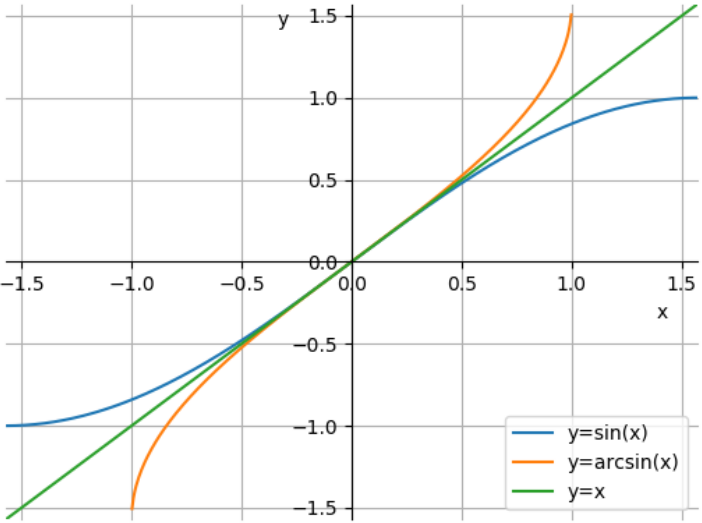
\includegraphics[width=.90\linewidth]{gfx/4/arcoseno.png}}
\caption{Arcoseno.}\label{fig:arcoseno}
\end{figure}

\begin{figure}[H]
{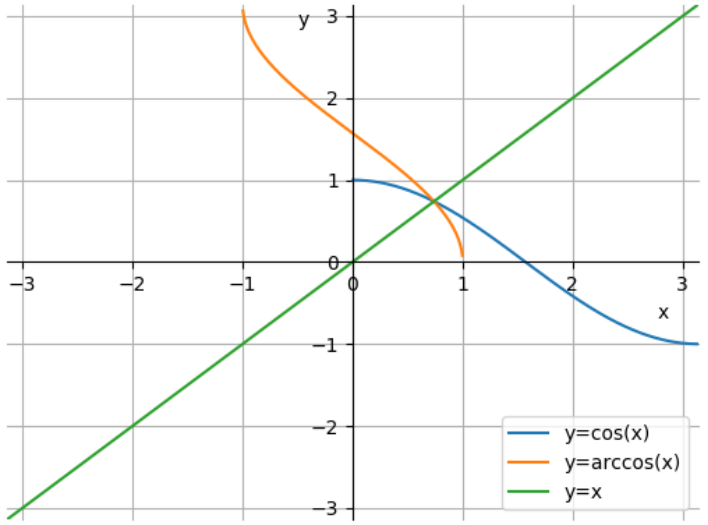
\includegraphics[width=.90\linewidth]{gfx/4/arcocoseno.png}
}
\caption{Arcocoseno.}\label{fig:arcocoseno}
\end{figure}

\begin{figure}[H]
{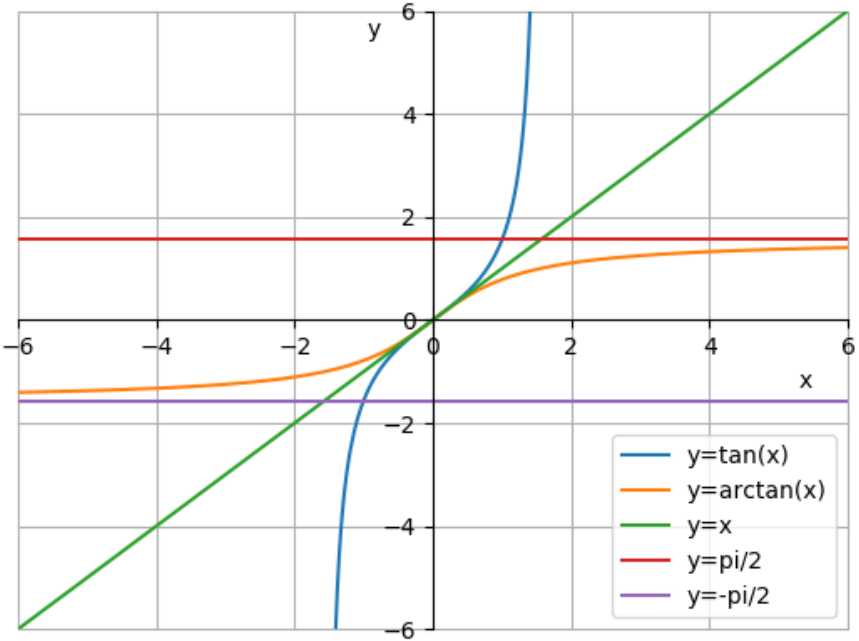
\includegraphics[width=.90\linewidth]{gfx/4/arcotangente.png}}
\caption{Arcotangente.}\label{fig:arcotangente}
\end{figure}
